\documentclass{report}

\usepackage{graphicx}
\usepackage{titlesec}
\usepackage{siunitx}
\usepackage[margin=1in]{geometry}
\usepackage{lscape}
\usepackage{rotating}
\usepackage{subcaption}
\usepackage{pdfpages}
\usepackage{changepage}
\usepackage{wrapfig}
\usepackage{hyperref}
\usepackage{listings}
\lstset{
	basicstyle=\small\ttfamily,
	columns=flexible,
	breaklines=true
}
\newcommand\tab[1][1cm]{\hspace*{#1}}


%This forces tables and figures placed in a section to stay
% in that section rather than floating away
\usepackage[section]{placeins}


%This suppresses each chapter displaying "Chapter X"
%\titleformat{\chapter}[display]
%{\normalfont\bfseries}{}{0pt}{\Large}

%This handles the formatting of chapter headings
% {left spacing}{before spacing}{after spacing}
\titlespacing*{\chapter}{0pt}{0pt}{0pt}

%This handles the formatting of section headings
% {left spacing}{before spacing}{after spacing}
\titlespacing*{\section}{0pt}{10pt}{0pt}

%This handles the formatting of subsection headings
% {left spacing}{before spacing}{after spacing}
\titlespacing*{\subsection}{0pt}{0pt}{5pt}

%This handles the formatting of subsubsection headings
% {left spacing}{before spacing}{after spacing}
\titlespacing*{\subsubsection}{0pt}{5pt}{0pt}


%Set up chapter
\title
{
	\textbf{{ROS-Gazebo-ErleRover \& Evo-ROS \\Installation and Usage Guide}\\
	{Michigan State University}\\}
	
\includegraphics{Images/MSU_Lab_Cover_Image.png}
}

\author{Glen Simon\\
Philip McKinley\\
Jared Moore\\
Anthony Clark}


%Current date will auto add here

\begin{document}
\maketitle

\newpage
%To update table of contents have to edit the line then build
\tableofcontents
\clearpage

\chapter{Introduction}
We introduce Evo-ROS, a framework combining evolutionary search and ROS/Gazebo-based simulation. The framework provides researchers in evolutionary robotics access to the extensive support for real-world components and capabilities developed by the ROS community. Conversely, Evo-ROS enables developers in the ROS community, and more broadly robotics researchers, to take advantage of evolutionary search during design. Evolutionary algorithms can be applied to many aspects of development, including optimal configuration and
placement of sensors and actuators, generation of compensatory behavior in case of failed/faulty components, and detection of “unlikely-but-possible” situations that might cause system failure.

The Evo-ROS framework separates the GA and simulation through a socket-based interface. Messages are sent from the GA to ROS/Gazebo instances, where the robot is evaluated. A fitness score is then returned through another socket back to the GA, where the generational loop is processed. In comparison to a typical ROS/Gazebo simulation, the primary extension a user needs to implement is mapping a genome into the robotic system. In our sample code, we show how to implement this approach for a simple Roomba-like robotic system as well as the more complex Erle-Rover robot.

To address performance concerns, Evo-ROS can exploit multiple levels of parallelism, including: deploying to (1) several physical machines; (2) several VMs on the same physical machine; (3) multiple ROS instances in the same VM; (4) multiple Gazebo simulations per ROS master; and (5) multiple, separate evaluations per Gazebo simulation (e.g., two robots completing tasks in separate zones–not interacting). The current Github repositories contain implementations of (2) with an Ardupilot based controller and (4) with a state machine based controller.

\chapter{Installation}
These installation directions are derived from the instructions provided by Erle Robotics found at\\ \href{http://docs.erlerobotics.com/simulation/configuring\_your\_environment}{http://docs.erlerobotics.com/simulation/configuring\_your\_environment}.
\\

It is recommended that this software be used on a machine running Ubuntu 14.04 64 bits.

ROS Indigo ONLY supports Saucy (13.10) and Trusty (14.04) for debian packages.

\section{Configuring your Ubuntu Machine}
These steps only have to be done once per machine.
\subsection{Install base packages}
\begin{lstlisting}
	sudo apt-get update
	sudo apt-get install gawk make git curl cmake -y
\end{lstlisting}

\subsection{Install dependencies for MAVProxy}
\begin{lstlisting}
	sudo apt-get install g++ python-pip python-matplotlib python-serial python-wxgtk2.8 python-scipy -y
	sudo apt-get install python-opencv python-numpy python-pyparsing ccache realpath libopencv-dev -y
\end{lstlisting}

\subsection{Install MAVProxy}
\begin{lstlisting}
	sudo pip install future
	sudo apt-get install libxml2-dev libxslt1-dev -y
	sudo pip2 install pymavlink catkin_pkg --upgrade
	sudo pip install -I MAVProxy==1.5.2
\end{lstlisting}

\subsection{Download and install ArUco}
\begin{enumerate}
	\item Download ArUco 1.3.0 from here \href{https://sourceforge.net/projects/aruco/files/1.3.0/aruco-1.3.0.tgz/download}{https://sourceforge.net/projects/aruco/files/1.3.0/aruco-1.3.0.tgz/download}
	
	\item Install ArUco

\begin{lstlisting}
	cd ~/Downloads # Replace this with your Download directory
	tar -xvzf aruco-1.3.0.tgz
	cd aruco-1.3.0/
	mkdir build && cd build
	cmake ..
	make
	sudo make install
\end{lstlisting}
\end{enumerate}

\subsection{Install ROS Indigo}
\subsubsection{Setup your computer to accept software from packages.ros.org, setup your keys and install (make sure your Debian package index is up-to-date):}
\begin{lstlisting}
	sudo sh -c 'echo "deb http://packages.ros.org/ros/ubuntu $(lsb_release -sc) main" > /etc/apt/sources.list.d/ros-latest.list'
	sudo apt-key adv --keyserver hkp://ha.pool.sks-keyservers.net --recv-key 0xB01FA116
	sudo apt-get update
\end{lstlisting}

\subsubsection{Install ROS package, build, and communication libraries:}
\begin{lstlisting}
	sudo apt-get install ros-indigo-ros-base -y
\end{lstlisting}

\subsubsection{Initialize rosdep. Before you can use ROS, you will need to initialize rosdep, which enables you to easily install system dependencies for source you want to compile and is required to run some core components in ROS.}
\begin{lstlisting}
	sudo rosdep init
	rosdep update
\end{lstlisting}

\subsubsection{It's convenient if the ROS environment variables are automatically added to your bash session every time a new shell is launched:}
\begin{lstlisting}
	echo "source /opt/ros/indigo/setup.bash" >> ~/.bashrc
	source ~/.bashrc
\end{lstlisting}

\subsubsection{Get rosinstall and some additional dependencies}
\begin{lstlisting}
	sudo apt-get    install python-rosinstall          \
	ros-indigo-octomap-msgs    \
	ros-indigo-joy             \
	ros-indigo-geodesy         \
	ros-indigo-octomap-ros     \
	ros-indigo-mavlink         \
	ros-indigo-control-toolbox \
	ros-indigo-transmission-interface \
	ros-indigo-joint-limits-interface \
	unzip -y
\end{lstlisting}

\subsubsection{Get RQT graph}
\begin{lstlisting}
sudo apt-get install ros-indigo-rqt
sudo apt-get install ros-indigo-rqt-common-plugins
\end{lstlisting}


\subsection{Install Gazebo}
\subsubsection{Setup your computer to accept software from packages.osrfoundation.org}
\begin{lstlisting}
	sudo sh -c 'echo "deb http://packages.osrfoundation.org/gazebo/ubuntu-stable `lsb_release -cs` main" > /etc/apt/sources.list.d/gazebo-stable.list'
\end{lstlisting}

\subsubsection{Setup keys}
\begin{lstlisting}
	wget http://packages.osrfoundation.org/gazebo.key -O - | sudo apt-key add -
\end{lstlisting}

\subsubsection{Install gazebo7}
\begin{lstlisting}
	sudo apt-get update
	sudo apt-get remove .*gazebo.* '.*sdformat.*' '.*ignition-math.*' && sudo apt-get update && sudo apt-get install gazebo7 libgazebo7-dev drcsim7 -y
\end{lstlisting}


\chapter{Configuring User Workspace}
These steps will have to be done for each user on a machine if they would like their own local copies of the source files.

\section{Download Ardupilot}
The ArduPilot project is an open source autopilot for drones, rovers, and other platforms. We'll be using its code to simulate the Unmanned ground vehicles (UGVs), specifically the Erle-Rover:
\subsection{Compile a specific branch of ardupilot}
\begin{lstlisting}
	mkdir -p ~/simulation; cd ~/simulation
	git clone https://github.com/erlerobot/ardupilot -b gazebo
\end{lstlisting}

\section{Download ErleRover\_Scripts directory}
This was created to ease the process of starting all of the required processes used to simulate the Erle Rover.
\begin{lstlisting}
	cd ~/simulation
	git clone https://github.com/gsimon2/ErleRover-Scripts.git
\end{lstlisting}
\subsection{Getting permission to push commits to the remote repo}
The above ErleRover-Scripts directory is a public repo and can freely be copied, but for access to submit changes please contact Glen Simon at glen.a.simon@gmail.com.

\section{Download ros\_gazebo\_python directory, which contains the BasicBot work. Optional}
\begin{lstlisting}
	cd ~/simulation
	git clone https://github.com/jaredmoore/ros_gazebo_python.git
\end{lstlisting}
\subsection{Getting permission to push commits to the remote repo}
The ros\_gazebo\_python directory is a public repo and can freely be copied, but for access to submit changes please contact Jared Moore at swiftfoottim@gmail.com.



\section{Create ROS workspace}
\subsection{Make workspace}
\begin{lstlisting}
	mkdir -p ~/simulation/ros_catkin_ws/src
\end{lstlisting}

\subsection{Initialize the workspace}
\begin{lstlisting}
	cd ~/simulation/ros_catkin_ws/src
	catkin_init_workspace
	cd ~/simulation/ros_catkin_ws
	catkin_make
	source devel/setup.bash
\end{lstlisting}

\subsection{Download ros\_catkin\_ws\_src which contains the development work for the MSU rover project}
\begin{lstlisting}
	cd ~/simulation/ros_catkin_ws
	git clone https://github.com/gsimon2/ros_catkin_ws_src.git
\end{lstlisting}

\subsubsection{Delete default src directory and replace with the downloaded one}
\begin{lstlisting}
	cd ~/simulation/ros_catkin_ws
	rm -r src
	mv ros_catkin_ws_src src
\end{lstlisting}

\subsubsection{Getting permission to push commits to the remote repo}
This is a public repo and can freely be copied, but for access to submit changes please contact Glen Simon at glen.a.simon@gmail.com.

\subsection{Compile the ros\_catkin\_ws workspace}
\begin{lstlisting}
	cd ~/simulation/ros_catkin_ws
	source devel/setup.bash
	catkin_make --pkg mav_msgs mavros_msgs gazebo_msgs
	catkin_make -j 4
\end{lstlisting}

\section{Download Gazebo models}
\begin{lstlisting}
	mkdir -p ~/.gazebo/models
	git clone https://github.com/erlerobot/erle_gazebo_models
	mv erle_gazebo_models/* ~/.gazebo/models
\end{lstlisting}

\section{Configuring .bashrc}
\subsection{Add ROS setup to bash}
	It's convenient if the ROS environment variables are automatically added to your bash session every time a new shell is launched.
\begin{lstlisting}
	echo "source /opt/ros/indigo/setup.bash" >> ~/.bashrc
	source ~/.bashrc
\end{lstlisting}

\subsection{Add ros\_catkin\_ws setup to bash}
	For ROS to find the packages provided in ros\_catkin\_ws we need to source the setup file every time. This is easier if we also add this to the bash file.
\begin{lstlisting}
	echo "source ~/simulation/ros_catkin_ws/devel/setup.bash" >> ~/.bashrc
	source ~/.bashrc
\end{lstlisting}






\chapter{Basic Simulation Usage}
\section{Basic Erle-Rover simulation}
This process will bring up the Erle-Rover in a blank world and allow you to manually enter throttle and yaw commands via the MAVProxy terminal.
\subsection{Manually starting all needed processes}
The process of starting all processes can be found in more detail at: \\ \href{http://docs.erlerobotics.com/simulation/vehicles/erle_rover/tutorial_1}{http://docs.erlerobotics.com/simulation/vehicles/erle\_rover/tutorial\_1}, but will be covered briefly here.
\subsubsection{Executing APMrover2}\label{MAVmanual}
This process requires two active terminals. 

In terminal one enter:
\begin{lstlisting}
	source ~/simulation/ros_catkin_ws/devel/setup.bash
	cd ~/simulation/ardupilot/APMrover2
	../Tools/autotest/sim_vehicle.sh -j 4 -f Gazebo
	# once MAVProxy has launched completely, load the parameters
	param load /[path_to_your_home_directory]/simulation/ardupilot/Tools/Frame_params/3DR_Rover.param
	# NOTE: replace [path_to_your_home_directory] with the actual path to your home directory.
	# Example: param load /home/john/simulation/ardupilot/Tools/Frame_params/3DR_Rover.param
\end{lstlisting}

In terminal two enter:
\begin{lstlisting}
	source ~/simulation/ros_catkin_ws/devel/setup.bash
	roslaunch ardupilot_sitl_gazebo_plugin rover_spawn.launch
\end{lstlisting}

This should start the Gazebo GUI and you should be able to see that the rover spawned in a blank world appearing similar to figure \ref{Erle-Rover-model}.

\begin{figure}[ht]
	\centering
	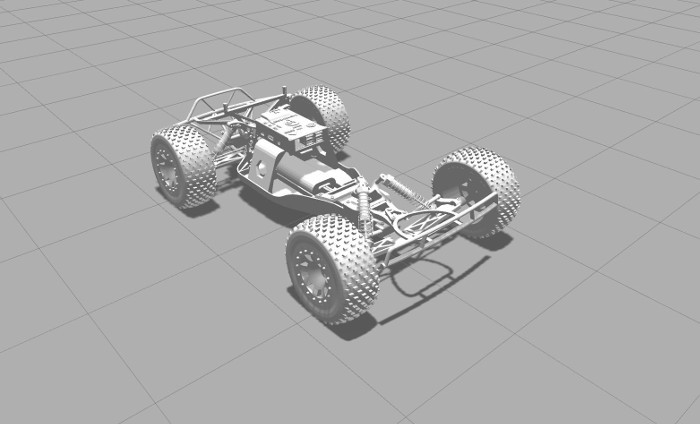
\includegraphics[scale = 0.35]{Images/rover}
	\caption{Erle-Rover model in Gazebo simulator}
	\label{Erle-Rover-model}
\end{figure}

\subsubsection{Controlling Erle-Rover using MAVProxy}
Make the rover move forward. In the first terminal execute:
\begin{lstlisting}
	# in the MAVProxy prompt:
	mode MANUAL
	param set SYSID_MYGCS 255
	rc 3 1900
\end{lstlisting}
Or backwards:
\begin{lstlisting}
	# in the MAVProxy prompt:
	rc 3 1200
\end{lstlisting}
What we are doing here is overriding the 3rd channel of the RC, which corresponds to the throttle. Values are from 1100 to 1900. 1500 is to stop the throttle; so values above 1500 will make the rover move forward, and values above 1500 backwards. The same principle applies to the yaw, which is in the 1st channel of the RC. Values above 1500 will make it turn right, and below 1500 left. For instance:
\begin{lstlisting}
	# in the MAVProxy prompt:
	rc 1 1400
\end{lstlisting}

Note that first we had to use ``param set SYSID\_MYGCS 255''. This tell MAVProxy where the source for rover commands are coming from. To control the rover manually via the MAVProxy terminal, this value must be set to 255. When using scripts to control the rover, this value must be set to 1.

\subsection{Using scripts to start simulation}
The above simulation can also be started using a script to make the start up process easier. To run the script enter the following commands:

\begin{lstlisting}
	cd ~/simulation/ErleRover-Scripts/
	./basic_sim.sh 
\end{lstlisting}
\label{startFPV}
This script also runs the ``start\_FPV'' script, which will bring up a window displaying a first person view from the rover's perspective. The ``start\_FPV'' script can be ran on its own anytime a simulation is running to show the first person view by running the following commands:
\begin{lstlisting}
cd ~/simulation/ErleRover-Scripts/
./start_FPV.sh 
\end{lstlisting}


\section{Starting MAVProxy via a script}\label{MAVscript}
MAVProxy is required when running any simulation of the rover and generally must manually be started prior to anything else. To make starting simulations easier, MAVProxy can be started via a script by using the following commands:
\begin{lstlisting}
	cd ~/simulation/ErleRover-Scripts/
	./start_MAVProxy.sh 
\end{lstlisting}

This will open an xterm window that sources the setup.bash file required to launch the Ardupilot SiTL software and execute Ardupilot's sim\_vehicle script with the rover parameters already loaded into it. The sim\_vehicle script will then launch MAVProxy in the xterm window and Ardupilot in a separate window, generally also xterm, but may vary depending on your system.



\section{Basic obstacle avoidance simulation using Erle Robotics script}
This process will bring up the rover in a basic maze and start a node running a basic obstacle avoidance algorithm provide by Erle Robotics which will lead the rover through the maze without crashing into the walls.

The process of starting all processes can be found in more detail at: \\ \href{http://docs.erlerobotics.com/simulation/vehicles/erle_rover/tutorial_2}{http://docs.erlerobotics.com/simulation/vehicles/erle\_rover/tutorial\_2}, but will be covered briefly here.

\subsection{Manually starting all needed processes}
To run this simulation three processes must be started:

\begin{enumerate}
	\item MAVProxy - This can be started manually, see terminal one in section \ref{MAVmanual}, or with a script, see section \ref{MAVscript}.
	\item The launch file - This can be done with the following command:
	\begin{lstlisting}
	roslaunch ardupilot_sitl_gazebo_plugin rover_maze.launch
	\end{lstlisting}
	\item The controller node - This can be done with the following command:
	\begin{lstlisting}
	rosrun erle_rover_explorer erle_rover_explorer.py
	\end{lstlisting}
\end{enumerate}

If this is done correctly you should see the rover spawn in a simple maze as can be seen in figure \ref{rovermaze1}. An overview of the maze can be seen in figure \ref{rovermaze2}.

\begin{figure}[ht]
	\centering
	\begin{subfigure}{.5\textwidth}
		\centering
		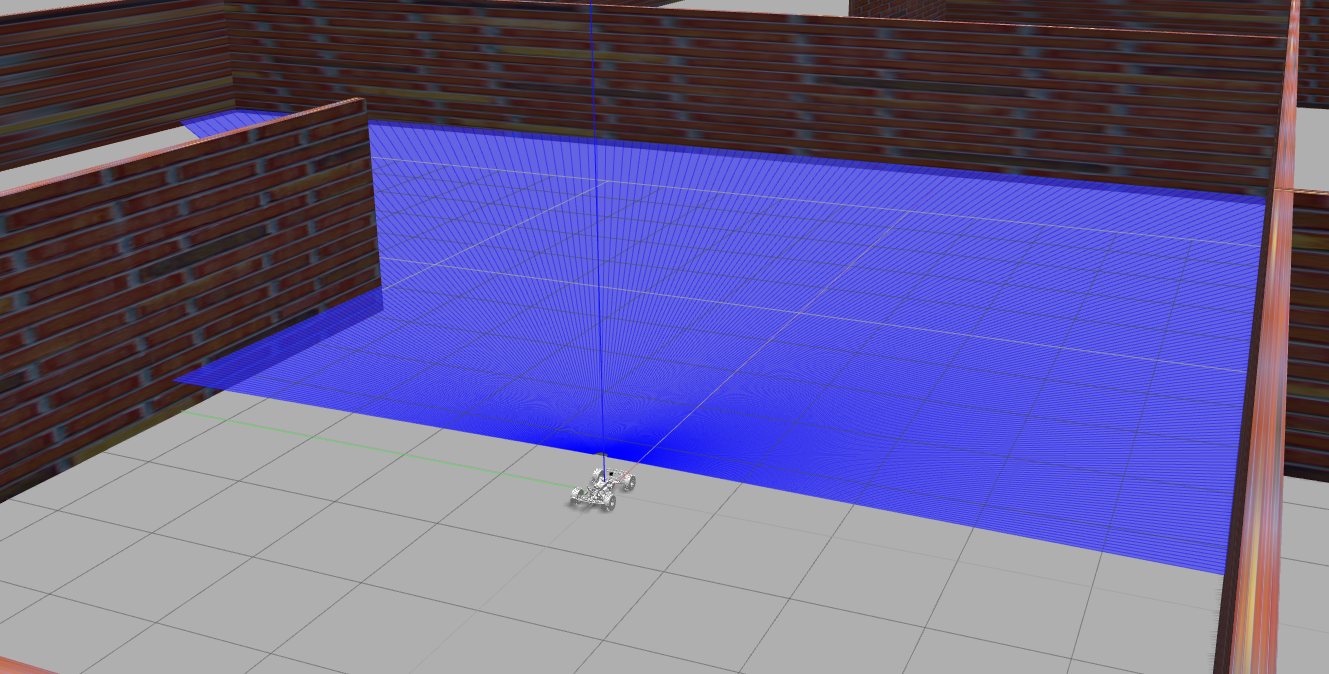
\includegraphics[width=0.9\linewidth]{Images/rover_maze_1}
		\caption{Erle-Rover in simple maze}
		\label{rovermaze1}
	\end{subfigure}%
	\begin{subfigure}{.5\textwidth}
		\centering
		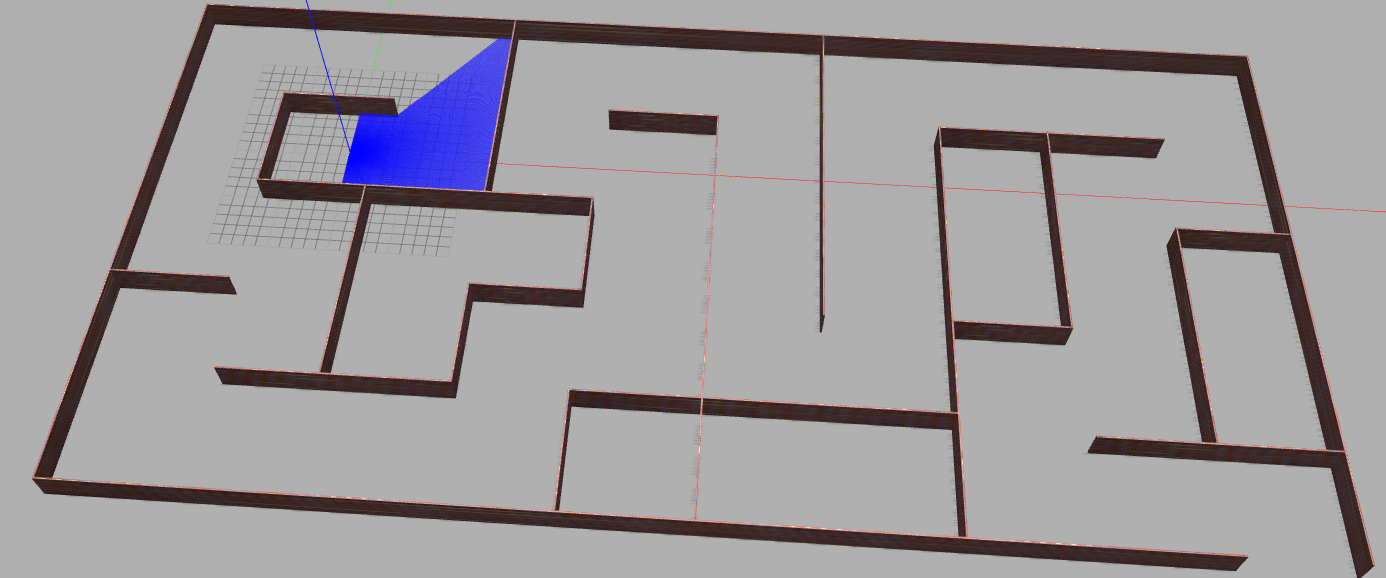
\includegraphics[width=1.05\linewidth]{Images/rover_maze_2}
		\caption{Simple maze overview}
		\label{rovermaze2}
	\end{subfigure}
\end{figure}

\subsubsection{Notes}
\begin{enumerate}
	\item There is no stopping condition for this simulation and the rover will just continue to drive straight once it has exited the maze.
	
	\item If the everything appears to have started correctly, but the rover is standing still in the maze, check to make sure MAVProxy is listening for commands on the right channel. For help with this issue see section \ref{changeMAVcommandSource}.
	
	\item The provided obstacle avoidance script also displays a window that represents the lidar scan and shows the current heading of the rover. An example of this can be seen in figure \ref{lidarRepresentation}.
	
	\item A first person view of the rover can be brought up by running the script. See section \ref{startFPV}.
\end{enumerate}

\begin{figure}[ht]
	\centering
	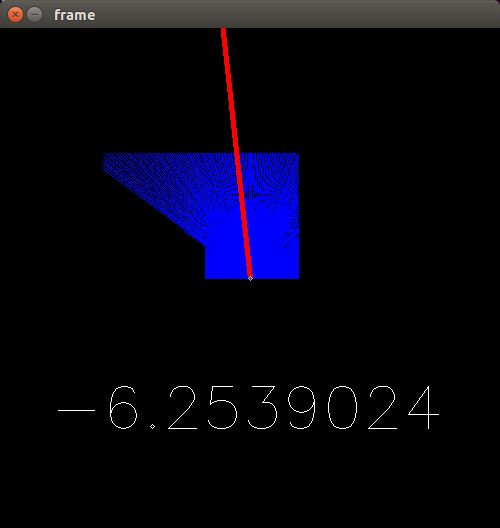
\includegraphics[scale=0.33]{Images/rover_maze_3}
	\caption{Lidar scan representation and current heading}
	\label{lidarRepresentation}
\end{figure}

\subsection{Using scripts to start simulation}
The above simulation can also be started using a script to make the start up process easier. To run the script enter the following commands:

\begin{lstlisting}
	cd ~/simulation/ErleRover-Scripts/
	./explorer_sim.sh 
\end{lstlisting}



%%%%%%%%%%%%%%%%%%%% Cutting this section until I can get it working again %%%%%%%%%%%%%
\iffalse
\section{Maze mapping using RViz}
The scan results from either an on board lidar or sonar sensor can be fed to RViz to generate an image of the maze as it is known to the rover. To do so, follow these steps:

\begin{enumerate}
	\item Start desired simulation - Launch all processes required for the simulation that you would like to map.
	
	\item 
\end{enumerate}

-----------------------------------------------------------------------------------------------\\
Experiencing issues with hector\_mapping mapping\_default.launch currently. Will finish this section when I resolve issues.\\
------------------------------------------------------------------------------------------------\\
\fi
%%%%%%%%%%%%%%%%%%%%%%%%%%%%%%%%%%%%%%%%%%%%%%%%%%%%%%%%%%%%%%%%%%%%%%%%%%%%%%%%%%%%%%%%%

\iffalse
\section{Line follower simulation}
Please follow directions provided at:
\href{http://docs.erlerobotics.com/simulation/vehicles/erle_rover/tutorial_3}{http://docs.erlerobotics.com/simulation/vehicles/erle\_rover/tutorial\_3}


\section{Object finder simulation}
\fi
%%%%%%%%%%%%%%%%%%%%%%%%%%%%%%%%%%%%%%%%%%%%%%%%%%%%%%%%%%%%%%%%%%%%%%%%%%%%%%%%%%%%%%%%%%%






\chapter{Evo-ROS}
\section{Motivation}
Evolutionary robotics (ER) applies the basic principles of genetic evolution to the design of robots through the application of the genetic algorithm (GA). An artificial genome specifies the robot’s control system and possibly aspects of its morphology (body). Individuals in a population are evaluated (typically in simulation) with respect to one or more tasks, with the best performing individuals selected to pass their genes
to the next generation. Evolutionary approaches have yielded effective controllers and physical designs for a variety of crawling, swimming, and flying robots [1, 5]. Our own research has applied evolutionary algorithms to optimize both morphology and control in aquatic and terrestrial robots. Evolving robot behavior and morphology is interesting in its own right, but from an engineering perspective, a major advantage of evolutionary search is the possible discovery of solutions (as well as potential problems) that the engineer might not otherwise have considered. 

Simulation is an essential component of evolutionary robotics, greatly reducing the time to evolve solutions while avoiding possible damage to physical robots. The ER community typically creates one-off simulation environments from a few different physics engines (e.g., ODE, Bullet, VoxCAD, Simulink) to conduct an experiment. Environments are sparse, generally featuring the robot and possibly a few obstacles. Tasks typically
comprise locomotion, navigation, and basic problem solving. Robots themselves contain only a few sensors, most often developed for the specific experiment being conducted. Hence, ER tasks are often limited by the scope of the simulation environment and how much time a developer has to code obstacles, sensors, and the platform itself. Models are not necessarily shareable between developers due to a lack of standardization. While many research questions can, and have, been answered by simple simulations, it becomes difficult to address more complex questions in these environments.

In contrast, the broader robotics community can address very complex tasks; the robotic systems utilize many sensor modalities to build a coherent understanding of their environment. By providing tested models of commercially available hardware, ROS/Gazebo provides a platform to study high-level behaviors while saving developer time during the design phase. Additionally, results have been shown to transfer to real robots,
potentially addressing the “reality-gap” often encountered in ER.

In the Evo-ROS project, we have developed an evolutionary framework that integrates ROS-based simulations for robot evaluation. Our current prototype includes ROS, Gazebo, Ardupilot and MAVROS. The primary goals of the project are twofold. First, the framework enables researchers in ER to take advantage ROS and related simulation tools. Second, it enables robot developers to employ evolutionary search during the design
process.






%%%%%%%%%%%%%%%%%%%%%%%%%%%%%%%%%%%%%%%%%%%%%%%%%%%%%%%%%%%%%%%%%%%%%%%%%%%%%%%%%%%%%%%
% Fill this out eventually
%%%%%%%%%%%%%%%%%%%%%%%%%%%%%%%%%%%%%%%%%%%%%%%%%%%%%%%%%%%%%%%%%%%%%%%%%%%%%%%%%%%%%%%
\iffalse
\section{Overview}


\begin{wrapfigure}{r}{0.6\textwidth}
	\centering 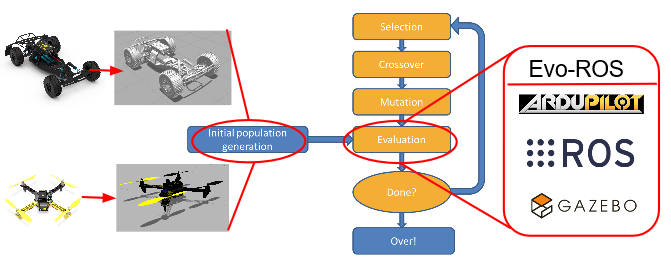
\includegraphics[width=0.6\textwidth]{Images/Evo-ROS_GA_Overview.png}
	\caption{Evo-ROS focuses on pulling the evaluation phase of the traditional GA sequence and reinforcing it with commercially available tools, such as: ROS, Gazebo, and Ardupilot.}
	\label{Evo-ROS_GA_Overview}	
\end{wrapfigure}

\begin{figure}[h]
	\centering
	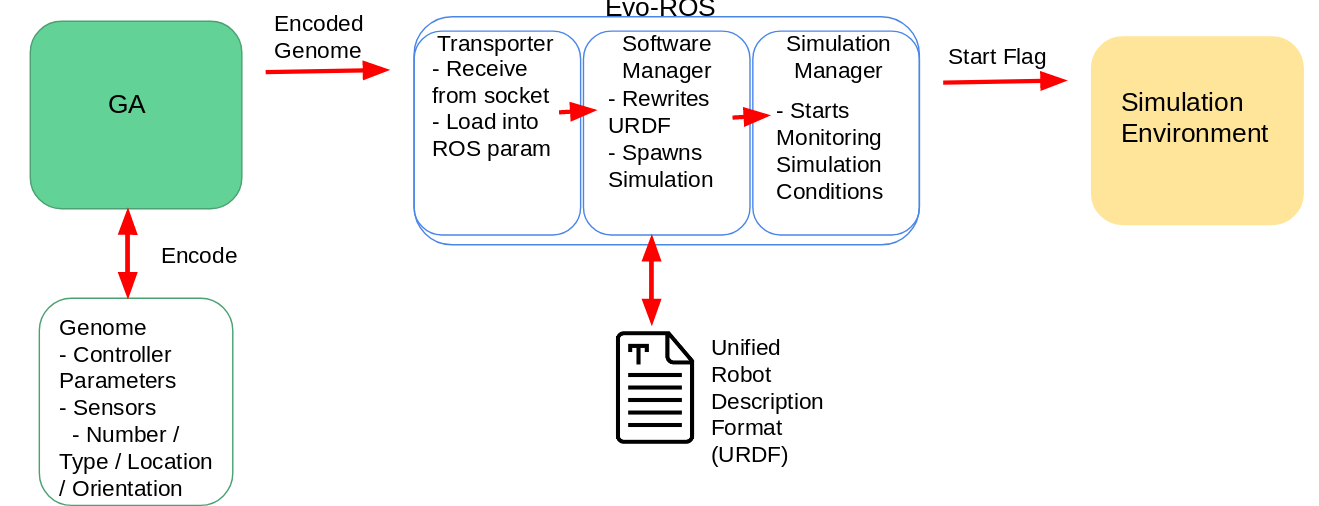
\includegraphics[scale=0.33]{Images/Evo-ROS_Forward_Workflow.png}
	\caption{This figure shows the forward progress of work flow that Evo-ROS performs to the simulated evaluation process.}
	\label{Evo-ROS_Forward_Workflow}
\end{figure}

\begin{figure}[h]
	\centering
	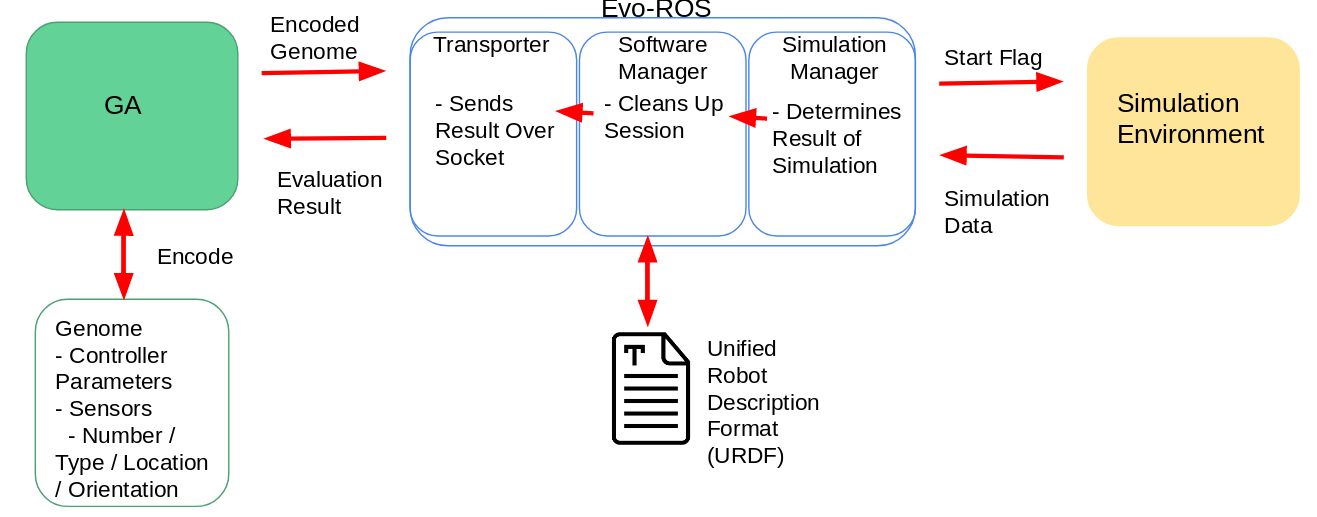
\includegraphics[scale=0.33]{Images/Evo-ROS_Backward_Workflow.png}
	\caption{This figure shows the work flow of Evo-ROS once the simulated evaluation is finished.}
	\label{Evo-ROS_Backward_Workflow}
\end{figure}
\fi 
%%%%%%%%%%%%%%%%%%%%%%%%%%%%%%%%%%%%%%%%%%%%%%%%%%%%%%%%%%%%%%%%%%%%%%%%%%%%%%%%%%%%%%%%%%%


\newpage
\section{Usage}
\subsection{Selecting and Configuring the GA}
\label{Selecting and Configuring the GA}

\begin{wrapfigure}{r}{0.45\textwidth}
	\centering 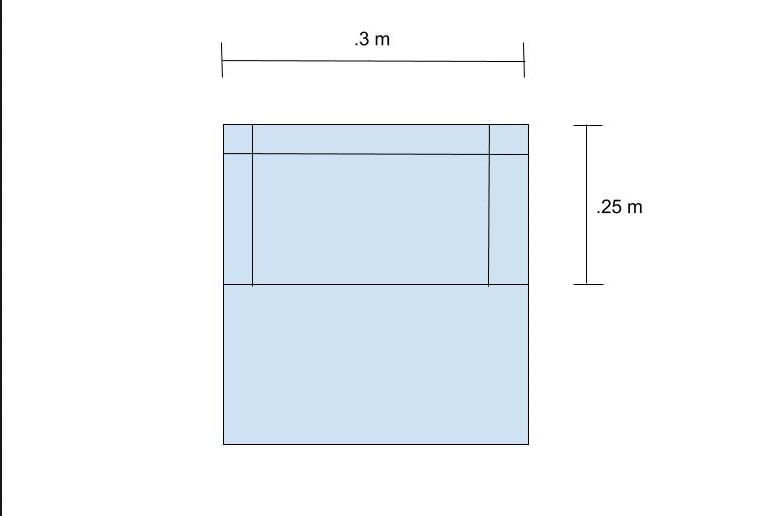
\includegraphics[width=0.45\textwidth]{Images/GA_Search_Space.png}
	\caption{The sonar positioning search space for the example GA. The search space is limited to the outside borders of the front half of the rover, so that there is ample room in the center for other sensors. For now, there is no need for sensing behind the rover, since it will only be moving forward.}
	\label{GA_Search_Space}	
\end{wrapfigure}

There are currently several different GA options that can be selected. For this example we are going to use the script ``symmetric\_variable\_number\_sonar\_GA\_server.py''. This script is used to explore the optimal placement of sonar sensors on an Erle-Rover. This particular does have some limitations to the search space. First, placement of the sensors is limited to the front half of the rover and must be pointed towards the front. This restriction is because for the controller that we are using, the rover will only be driving in the forward direction and thus will have no need for rear facing sensors. The second limitation, is that sensors are limited to the outside border of the front half. This limitation is to allow ample room in the center of the rover for the placement of the battery and other electronics. Lastly, since the evoluation of symmetric patterns is seen often in nature, the GA will force symmetry over the Y-axis of the rover for the placement of any sensors. That is, if there is a sensor selected to be placed at the front right corner of the rover at a 10 degree angle, then there will be a matching sensor placed at the front left corner of the rover at a -10 degree angle.

Once the GA is selected there are a few configuration options that should be observed. The configuration file can be opened by using the following commands:
\begin{lstlisting}
	cd ~/simulation/ros_catkin_ws/src/evo_ros/config/
	vim default_config.yml  
\end{lstlisting}

This file contains the default configuration options for many aspects of Evo-ROS, but currently we are only interested in those that deal with the GA portion. The ``ga\_server'' section can be found towards the top of the file and contains different parameters for the GA, such as: the tournament size, population size, generation count, log file name, and others.

After you are satisfied with the parameters being used the GA can be started by navigating to the GA directory by using the following commands:
 \begin{lstlisting}
	 cd ~/simulation/ros_catkin_ws/src/evo_ros/GA/
 \end{lstlisting}
 
Next you can see the running options for the GA by using the ``-h'' flag as shown below:
 \begin{lstlisting}
	python symmetric_variable_number_sonar_GA_server.py -h
 \end{lstlisting}
 
 Or you can start the GA in debugging mode with the following command:
\begin{lstlisting}
  python symmetric_variable_number_sonar_GA_server.py -d -ip 127.0.0.1
\end{lstlisting}
  
 It is recommend to start the GA in debugging mode so that extra output is printed to the terminal, which allows to verify parameters and track progression better. Since the GA uses a comparatively low amount of CPU time as compared to the evaluation software, the extra printed output has a negligible effect to running time.
 
 Also note that we specified the IP address that the GA should use to send out the genomes. By default, if this parameter is left blank, the GA will auto-assign it to be the IP address of the current machine.
 
 If all is running correctly, the terminal output should appear close to what is shown in figure \ref{GA_terminal_output}.
 
 \begin{figure}[h]
 	\centering
 	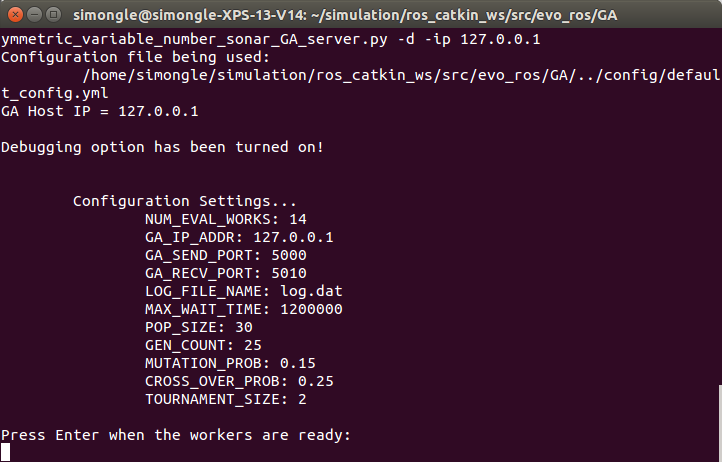
\includegraphics[scale=0.33]{Images/GA_Terminal_Output.png}
 	\caption{Expected output from starting the GA with the debugging options turned on.}
 	\label{GA_terminal_output}
 \end{figure}



\subsection{Evo-ROS Configuration Options}
There are a number of other Evo-ROS configuration options that can be found in the configuration file descripbed in section \ref{Selecting and Configuring the GA}. The configuration file is broken into sections, each corresponding to a major part of the Evo-ROS framework. These sections include: 

\begin{itemize}
	\item sonar\_filter
		\subitem This process is responsible for collecting all raw data from the sonar sensors in Gazebo and relying the information onto a ``/sonar\#\_filtered'' topic. This allows different filters to be applied to the raw data. One use of this is to apply different failure models to the sensors before the information is passed onto the robot's controller.
	\item software\_manager
		\subitem The software\_manager process is responsible for spawning and managing all of the other required processes within Evo\_ROS. It is in this set of configuration options that most of the customizations will be made. Here you can select things like: what launch files to use, as well as, which simulation managers and robotic controllers to use.
	\item transporter
		\subitem The transporter process creates and maintains the connection to the external GA process. 
	\item sim\_manager
		\subitem The sim\_manager (short for simulation manager) is the process that is responsible 
\end{itemize}


\subsection{Starting Evo-ROS}
The process of starting Evo-ROS is relatively simple once the configuration options have been set. For this example, no configuration options have to be changed. To start Evo-ROS, just has to start the ``software\_manager'' script and the rest will be managed automatically. The 	``software\_manager'' script can be started by entering the following command into a new instance of the terminal:
\begin{lstlisting}
	rosrun evo_ros software_manager.py -ip 127.0.0.1 -d -gui
\end{lstlisting}

Please note that the ``-ip'' flag is being passed to the software\_manager with the same IP address that we that gave the GA so that the two will be connected. 

The debugging option (``-d'' flag) is also set so that each process will spawn in it own window. This allows for easier understanding of what is all happening, but should not be used in production runs as it goes have an impact on the running time.

The ``-gui'' flag is set as well. This option tell Gazebo that it should bring up its full GUI when it is launched, allowing you to view the rover in the simulated environment. This option should not be used in production runs, as it also impacts the running time.

As with any Evo-ROS process, the software\_manager can be started with the ``-h'' help flag to display all possible options.

After the software\_manager has started, one additional terminal should spawn running the Evo-ROS transporter. At this point you should have terminals open for the GA, software\_manager, and the transporter. The Evo-ROS processes should be waiting to receive information for the GA, while the GA is waiting for you to give it the okay to start sending information.



\begin{figure}[h]
	\centering
 	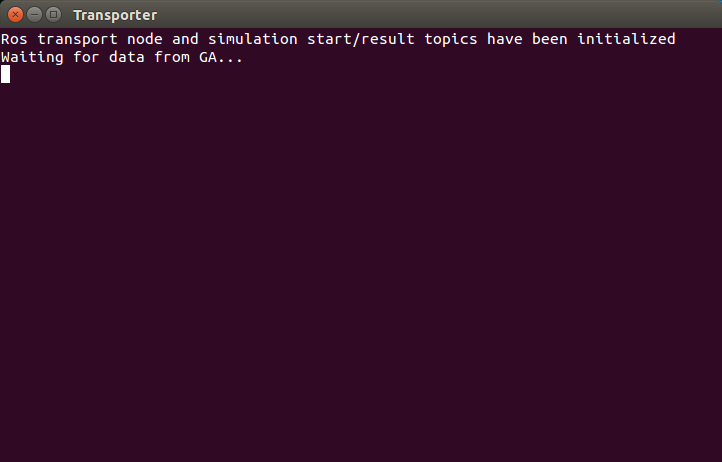
\includegraphics[scale=0.33]{Images/transporter_term_image.png}
 	\caption{Expected output of the transporter terminal.}
 	\label{transporter_term_image}
\end{figure}
 
\begin{figure}[h]
	\centering
  	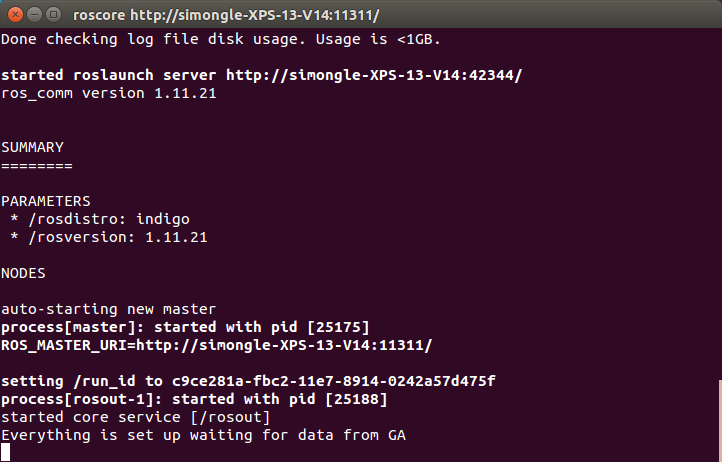
\includegraphics[scale=0.33]{Images/software_manager_term_image.png}
  	\caption{Expected output of the software manager terminal.}
  	\label{software_manager_term_image}
\end{figure}


\subsection{Using Evo-ROS}
Once both the GA and the software\_manager have been started, you simply have the give the GA permission to start sending information by pressing ``enter'' in that terminal. Upon pressing ``enter'' you should see the genomes from the GA being sent out. In the transporter window you will see one being received and being passed to the software\_manager. The software\_manager will then begin its process of setting up the simulated evaluation environment. This setup process includes spawning multiple xterm instances as well as a Gazebo instance (assuming the ``-d'' and ``-gui'' flags are set). This spawning process could take up to several minutes.

After the set up process has been completed, you should be able to view the rover in the Gazebo environment. The controller for the rover will automatically be started and after 10-20 seconds the rover should start its mission. During this time the simulation\_manager process will be monitoring its progression through the maze and monitoring for ending criteria, such as: a crash, mission completion, or a max time limit is reached. When an ending criteria is met, the results of the evaluation will be sent back the to GA, where a fitness can be assigned to the individual.

This instance of Evo-ROS will continue to receive individuals to be evaluated until the GA is either finished or canceled. 
	



\chapter{Troubleshooting}
\section{Rover is not responding to either manual or scripted commands}\label{changeMAVcommandSource}
The most common issue for the rover not responding to commands as expected is that MAVProxy is listening for commands on the wrong channel. To check for this enter the following command into the MAVProxy terminal to check which channel is currently being listened to for commands:
\begin{lstlisting}
	param show SYSID_MYGCS
\end{lstlisting}

If the returned value is 1.0, MAVProxy is listening for commands from a scripted controller comminicating using a ROS topic.

If the returned value is 255.0, MAVProxy is waiting for commands manually entered into the MAVProxy terminal. \\

To change the channel that MAVProxy is listening on use the following command:

\begin{lstlisting}
	param set SYSID_MYGCS {value}
\end{lstlisting}

where value is between 1 and 255.\\

Note: MAVProxy must be connected to the rover, either a physical rover or a ROS node acting as the rover, for these commands to work.

\begin{figure}[ht]
	\centering
	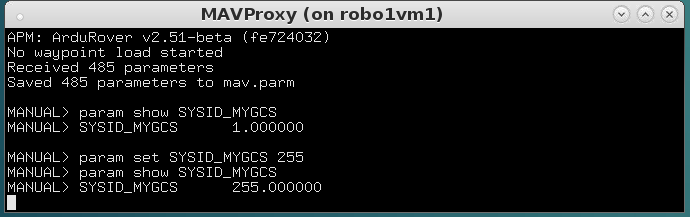
\includegraphics{Images/MAVcommandSourse}
	\caption{Checking MAVProxy command source}
\end{figure}



\end{document}
